\documentclass[1p]{elsarticle_modified}
%\bibliographystyle{elsarticle-num}

%\usepackage[colorlinks]{hyperref}
%\usepackage{abbrmath_seonhwa} %\Abb, \Ascr, \Acal ,\Abf, \Afrak
\usepackage{amsfonts}
\usepackage{amssymb}
\usepackage{amsmath}
\usepackage{amsthm}
\usepackage{scalefnt}
\usepackage{amsbsy}
\usepackage{kotex}
\usepackage{caption}
\usepackage{subfig}
\usepackage{color}
\usepackage{graphicx}
\usepackage{xcolor} %% white, black, red, green, blue, cyan, magenta, yellow
\usepackage{float}
\usepackage{setspace}
\usepackage{hyperref}

\usepackage{tikz}
\usetikzlibrary{arrows}

\usepackage{multirow}
\usepackage{array} % fixed length table
\usepackage{hhline}

%%%%%%%%%%%%%%%%%%%%%
\makeatletter
\renewcommand*\env@matrix[1][\arraystretch]{%
	\edef\arraystretch{#1}%
	\hskip -\arraycolsep
	\let\@ifnextchar\new@ifnextchar
	\array{*\c@MaxMatrixCols c}}
\makeatother %https://tex.stackexchange.com/questions/14071/how-can-i-increase-the-line-spacing-in-a-matrix
%%%%%%%%%%%%%%%

\usepackage[normalem]{ulem}

\newcommand{\msout}[1]{\ifmmode\text{\sout{\ensuremath{#1}}}\else\sout{#1}\fi}
%SOURCE: \msout is \stkout macro in https://tex.stackexchange.com/questions/20609/strikeout-in-math-mode

\newcommand{\cancel}[1]{
	\ifmmode
	{\color{red}\msout{#1}}
	\else
	{\color{red}\sout{#1}}
	\fi
}

\newcommand{\add}[1]{
	{\color{blue}\uwave{#1}}
}

\newcommand{\replace}[2]{
	\ifmmode
	{\color{red}\msout{#1}}{\color{blue}\uwave{#2}}
	\else
	{\color{red}\sout{#1}}{\color{blue}\uwave{#2}}
	\fi
}

\newcommand{\Sol}{\mathcal{S}} %segment
\newcommand{\D}{D} %diagram
\newcommand{\A}{\mathcal{A}} %arc


%%%%%%%%%%%%%%%%%%%%%%%%%%%%%5 test

\def\sl{\operatorname{\textup{SL}}(2,\Cbb)}
\def\psl{\operatorname{\textup{PSL}}(2,\Cbb)}
\def\quan{\mkern 1mu \triangleright \mkern 1mu}

\theoremstyle{definition}
\newtheorem{thm}{Theorem}[section]
\newtheorem{prop}[thm]{Proposition}
\newtheorem{lem}[thm]{Lemma}
\newtheorem{ques}[thm]{Question}
\newtheorem{cor}[thm]{Corollary}
\newtheorem{defn}[thm]{Definition}
\newtheorem{exam}[thm]{Example}
\newtheorem{rmk}[thm]{Remark}
\newtheorem{alg}[thm]{Algorithm}

\newcommand{\I}{\sqrt{-1}}
\begin{document}

%\begin{frontmatter}
%
%\title{Boundary parabolic representations of knots up to 8 crossings}
%
%%% Group authors per affiliation:
%\author{Yunhi Cho} 
%\address{Department of Mathematics, University of Seoul, Seoul, Korea}
%\ead{yhcho@uos.ac.kr}
%
%
%\author{Seonhwa Kim} %\fnref{s_kim}}
%\address{Center for Geometry and Physics, Institute for Basic Science, Pohang, 37673, Korea}
%\ead{ryeona17@ibs.re.kr}
%
%\author{Hyuk Kim}
%\address{Department of Mathematical Sciences, Seoul National University, Seoul 08826, Korea}
%\ead{hyukkim@snu.ac.kr}
%
%\author{Seokbeom Yoon}
%\address{Department of Mathematical Sciences, Seoul National University, Seoul, 08826,  Korea}
%\ead{sbyoon15@snu.ac.kr}
%
%\begin{abstract}
%We find all boundary parabolic representation of knots up to 8 crossings.
%
%\end{abstract}
%\begin{keyword}
%    \MSC[2010] 57M25 
%\end{keyword}
%
%\end{frontmatter}

%\linenumbers
%\tableofcontents
%
\newcommand\colored[1]{\textcolor{white}{\rule[-0.35ex]{0.8em}{1.4ex}}\kern-0.8em\color{red} #1}%
%\newcommand\colored[1]{\textcolor{white}{ #1}\kern-2.17ex	\textcolor{white}{ #1}\kern-1.81ex	\textcolor{white}{ #1}\kern-2.15ex\color{red}#1	}

{\Large $\underline{12a_{0105}~(K12a_{0105})}$}

\setlength{\tabcolsep}{10pt}
\renewcommand{\arraystretch}{1.6}
\vspace{1cm}\begin{tabular}{m{100pt}>{\centering\arraybackslash}m{274pt}}
\multirow{5}{120pt}{
	\centering
	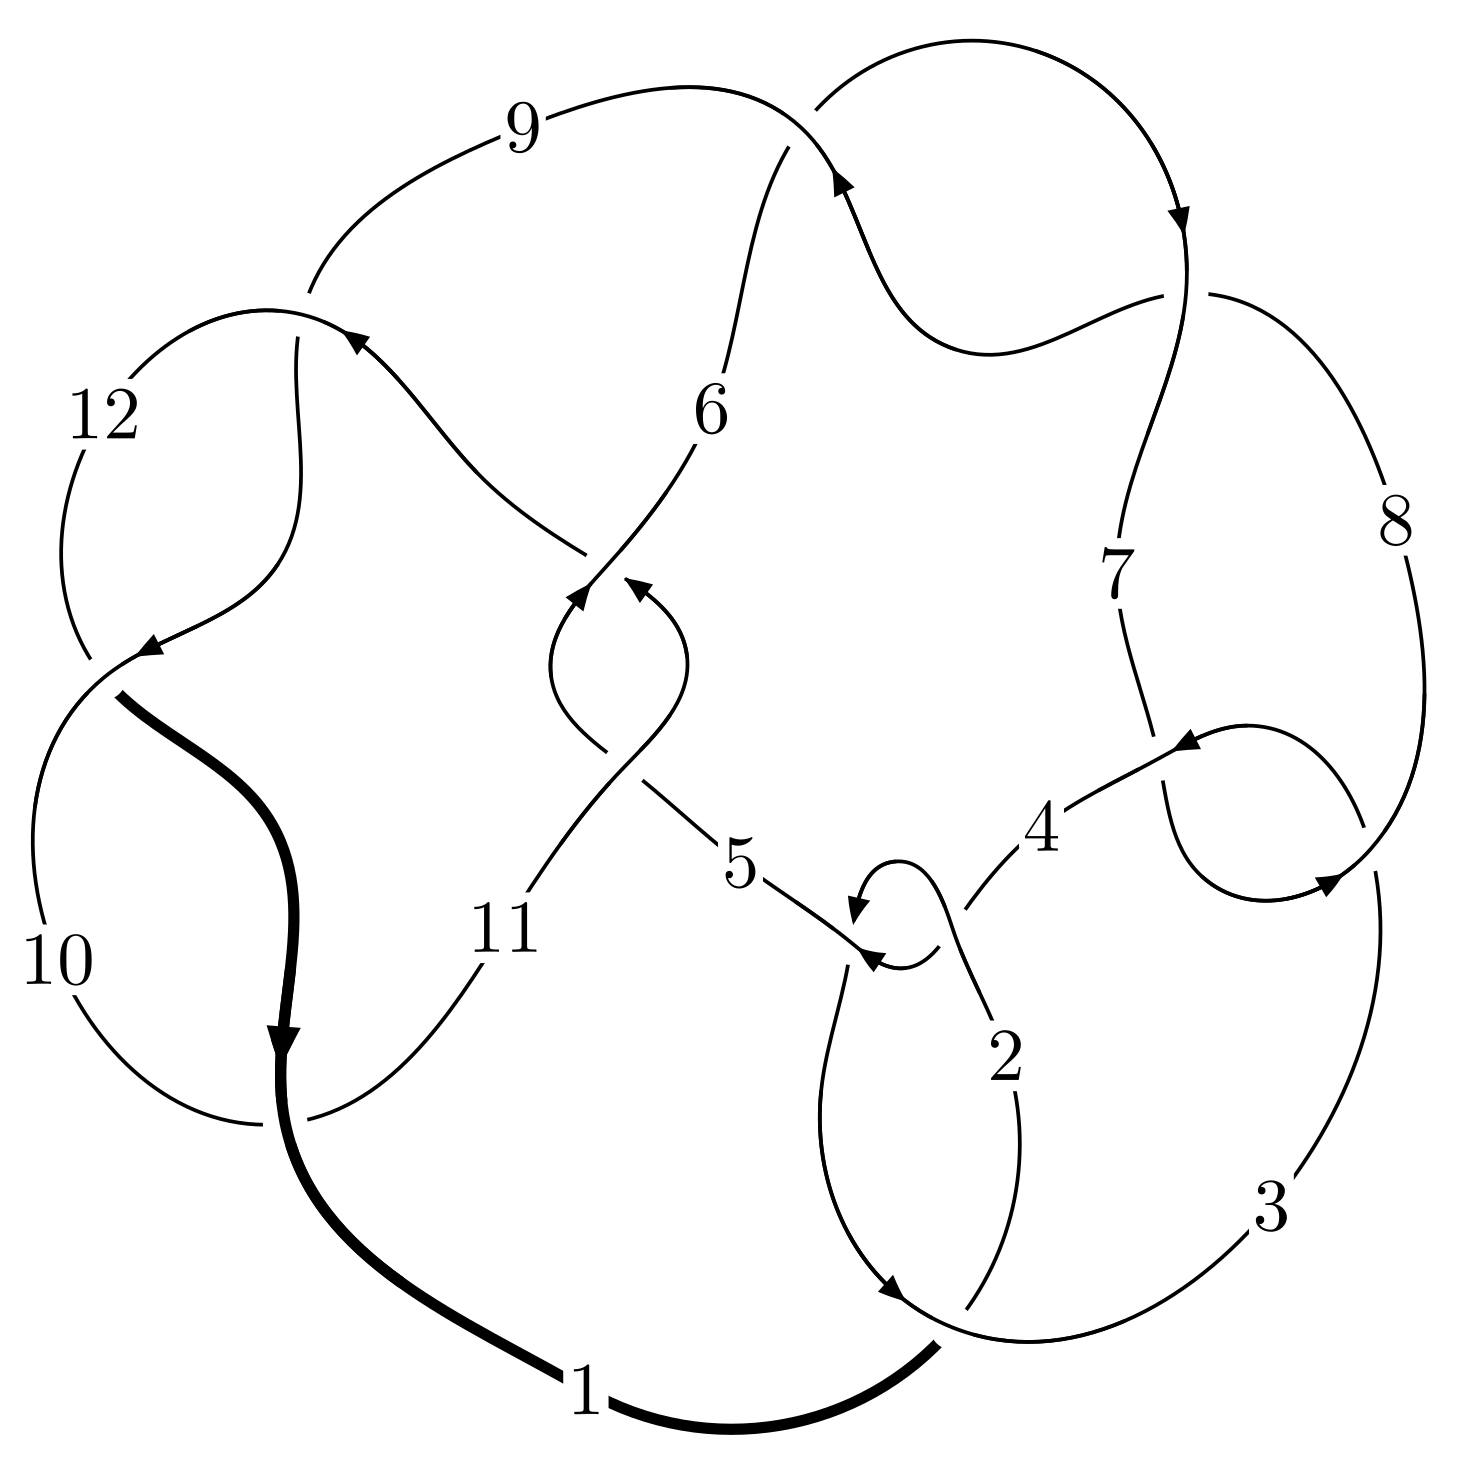
\includegraphics[width=112pt]{../../../GIT/diagram.site/Diagrams/png/906_12a_0105.png}\\
\ \ \ A knot diagram\footnotemark}&
\allowdisplaybreaks
\textbf{Linearized knot diagam} \\
\cline{2-2}
 &
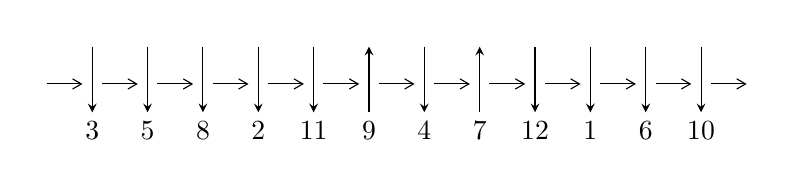
\begin{tikzpicture}[x=20pt, y=17pt]
	% nodes
	\node (C0) at (0, 0) {};
	\node (C1) at (1, 0) {};
	\node (C1U) at (1, +1) {};
	\node (C1D) at (1, -1) {3};

	\node (C2) at (2, 0) {};
	\node (C2U) at (2, +1) {};
	\node (C2D) at (2, -1) {5};

	\node (C3) at (3, 0) {};
	\node (C3U) at (3, +1) {};
	\node (C3D) at (3, -1) {8};

	\node (C4) at (4, 0) {};
	\node (C4U) at (4, +1) {};
	\node (C4D) at (4, -1) {2};

	\node (C5) at (5, 0) {};
	\node (C5U) at (5, +1) {};
	\node (C5D) at (5, -1) {11};

	\node (C6) at (6, 0) {};
	\node (C6U) at (6, +1) {};
	\node (C6D) at (6, -1) {9};

	\node (C7) at (7, 0) {};
	\node (C7U) at (7, +1) {};
	\node (C7D) at (7, -1) {4};

	\node (C8) at (8, 0) {};
	\node (C8U) at (8, +1) {};
	\node (C8D) at (8, -1) {7};

	\node (C9) at (9, 0) {};
	\node (C9U) at (9, +1) {};
	\node (C9D) at (9, -1) {12};

	\node (C10) at (10, 0) {};
	\node (C10U) at (10, +1) {};
	\node (C10D) at (10, -1) {1};

	\node (C11) at (11, 0) {};
	\node (C11U) at (11, +1) {};
	\node (C11D) at (11, -1) {6};

	\node (C12) at (12, 0) {};
	\node (C12U) at (12, +1) {};
	\node (C12D) at (12, -1) {10};
	\node (C13) at (13, 0) {};

	% arrows
	\draw[->,>={angle 60}]
	(C0) edge (C1) (C1) edge (C2) (C2) edge (C3) (C3) edge (C4) (C4) edge (C5) (C5) edge (C6) (C6) edge (C7) (C7) edge (C8) (C8) edge (C9) (C9) edge (C10) (C10) edge (C11) (C11) edge (C12) (C12) edge (C13) ;	\draw[->,>=stealth]
	(C1U) edge (C1D) (C2U) edge (C2D) (C3U) edge (C3D) (C4U) edge (C4D) (C5U) edge (C5D) (C6D) edge (C6U) (C7U) edge (C7D) (C8D) edge (C8U) (C9U) edge (C9D) (C10U) edge (C10D) (C11U) edge (C11D) (C12U) edge (C12D) ;
	\end{tikzpicture} \\
\hhline{~~} \\& 
\textbf{Solving Sequence} \\ \cline{2-2} 
 &
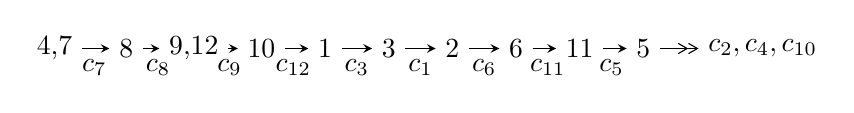
\begin{tikzpicture}[x=23pt, y=7pt]
	% node
	\node (A0) at (-1/8, 0) {4,7};
	\node (A1) at (1, 0) {8};
	\node (A2) at (33/16, 0) {9,12};
	\node (A3) at (25/8, 0) {10};
	\node (A4) at (33/8, 0) {1};
	\node (A5) at (41/8, 0) {3};
	\node (A6) at (49/8, 0) {2};
	\node (A7) at (57/8, 0) {6};
	\node (A8) at (65/8, 0) {11};
	\node (A9) at (73/8, 0) {5};
	\node (C1) at (1/2, -1) {$c_{7}$};
	\node (C2) at (3/2, -1) {$c_{8}$};
	\node (C3) at (21/8, -1) {$c_{9}$};
	\node (C4) at (29/8, -1) {$c_{12}$};
	\node (C5) at (37/8, -1) {$c_{3}$};
	\node (C6) at (45/8, -1) {$c_{1}$};
	\node (C7) at (53/8, -1) {$c_{6}$};
	\node (C8) at (61/8, -1) {$c_{11}$};
	\node (C9) at (69/8, -1) {$c_{5}$};
	\node (A10) at (11, 0) {$c_{2},c_{4},c_{10}$};

	% edge
	\draw[->,>=stealth]	
	(A0) edge (A1) (A1) edge (A2) (A2) edge (A3) (A3) edge (A4) (A4) edge (A5) (A5) edge (A6) (A6) edge (A7) (A7) edge (A8) (A8) edge (A9) ;
	\draw[->>,>={angle 60}]	
	(A9) edge (A10);
\end{tikzpicture} \\ 

\end{tabular} \\

\footnotetext{
The image of knot diagram is generated by the software ``\textbf{Draw programme}" developed by Andrew Bartholomew(\url{http://www.layer8.co.uk/maths/draw/index.htm\#Running-draw}), where we modified some parts for our purpose(\url{https://github.com/CATsTAILs/LinksPainter}).
}\phantom \\ \newline 
\centering \textbf{Ideals for irreducible components\footnotemark of $X_{\text{par}}$} 
 
\begin{align*}
I^u_{1}&=\langle 
-1.55045\times10^{70} u^{75}-2.21319\times10^{69} u^{74}+\cdots+1.11366\times10^{71} b-4.15501\times10^{71},\\
\phantom{I^u_{1}}&\phantom{= \langle  }1.74213\times10^{71} u^{75}+4.23795\times10^{71} u^{74}+\cdots+2.22733\times10^{71} a+2.49538\times10^{71},\;u^{76}+2 u^{75}+\cdots-4 u-4\rangle \\
I^u_{2}&=\langle 
u^2+b,\;u^8-2 u^7+3 u^6-3 u^5+4 u^4-4 u^3+4 u^2+a-2 u+2,\;u^9- u^8+2 u^7- u^6+3 u^5- u^4+2 u^3+u+1\rangle \\
\\
I^v_{1}&=\langle 
a,\;b+v+2,\;v^2+3 v+1\rangle \\
\end{align*}
\raggedright * 3 irreducible components of $\dim_{\mathbb{C}}=0$, with total 87 representations.\\
\footnotetext{All coefficients of polynomials are rational numbers. But the coefficients are sometimes approximated in decimal forms when there is not enough margin.}
\newpage
\renewcommand{\arraystretch}{1}
\centering \section*{I. $I^u_{1}= \langle -1.55\times10^{70} u^{75}-2.21\times10^{69} u^{74}+\cdots+1.11\times10^{71} b-4.16\times10^{71},\;1.74\times10^{71} u^{75}+4.24\times10^{71} u^{74}+\cdots+2.23\times10^{71} a+2.50\times10^{71},\;u^{76}+2 u^{75}+\cdots-4 u-4 \rangle$}
\flushleft \textbf{(i) Arc colorings}\\
\begin{tabular}{m{7pt} m{180pt} m{7pt} m{180pt} }
\flushright $a_{4}=$&$\begin{pmatrix}0\\u\end{pmatrix}$ \\
\flushright $a_{7}=$&$\begin{pmatrix}1\\0\end{pmatrix}$ \\
\flushright $a_{8}=$&$\begin{pmatrix}1\\u^2\end{pmatrix}$ \\
\flushright $a_{9}=$&$\begin{pmatrix}u^2+1\\u^2\end{pmatrix}$ \\
\flushright $a_{12}=$&$\begin{pmatrix}-0.782160 u^{75}-1.90270 u^{74}+\cdots+0.520711 u-1.12035\\0.139220 u^{75}+0.0198730 u^{74}+\cdots+6.72179 u+3.73093\end{pmatrix}$ \\
\flushright $a_{10}=$&$\begin{pmatrix}-1.01250 u^{75}-2.27723 u^{74}+\cdots-4.68125 u-3.11714\\-0.533374 u^{75}-1.25764 u^{74}+\cdots-10.8152 u-5.20956\end{pmatrix}$ \\
\flushright $a_{1}=$&$\begin{pmatrix}-0.650123 u^{75}-1.66160 u^{74}+\cdots+1.45358 u-1.64453\\-0.487576 u^{75}-0.547614 u^{74}+\cdots-12.0164 u-5.53730\end{pmatrix}$ \\
\flushright $a_{3}=$&$\begin{pmatrix}u\\u^3+u\end{pmatrix}$ \\
\flushright $a_{2}=$&$\begin{pmatrix}-0.841202 u^{75}-1.99701 u^{74}+\cdots-1.61931 u-3.16059\\-0.379305 u^{75}-0.461175 u^{74}+\cdots-15.6666 u-6.86635\end{pmatrix}$ \\
\flushright $a_{6}=$&$\begin{pmatrix}u^4+u^2+1\\u^4\end{pmatrix}$ \\
\flushright $a_{11}=$&$\begin{pmatrix}-0.866472 u^{75}-2.19326 u^{74}+\cdots+4.35819 u+0.256226\\0.137653 u^{75}+0.177442 u^{74}+\cdots+6.46899 u+3.72188\end{pmatrix}$ \\
\flushright $a_{5}=$&$\begin{pmatrix}-0.389207 u^{75}-1.15743 u^{74}+\cdots+9.42404 u+2.44734\\0.260915 u^{75}+0.504172 u^{74}+\cdots+7.97047 u+4.09188\end{pmatrix}$\\&\end{tabular}
\flushleft \textbf{(ii) Obstruction class $= -1$}\\~\\
\flushleft \textbf{(iii) Cusp Shapes $= -0.431038 u^{75}-2.36353 u^{74}+\cdots+19.7107 u-1.47053$}\\~\\
\newpage\renewcommand{\arraystretch}{1}
\flushleft \textbf{(iv) u-Polynomials at the component}\newline \\
\begin{tabular}{m{50pt}|m{274pt}}
Crossings & \hspace{64pt}u-Polynomials at each crossing \\
\hline $$\begin{aligned}c_{1}\end{aligned}$$&$\begin{aligned}
&u^{76}+44 u^{75}+\cdots+64 u+1
\end{aligned}$\\
\hline $$\begin{aligned}c_{2},c_{4}\end{aligned}$$&$\begin{aligned}
&u^{76}-4 u^{75}+\cdots-32 u^2+1
\end{aligned}$\\
\hline $$\begin{aligned}c_{3},c_{7}\end{aligned}$$&$\begin{aligned}
&u^{76}+2 u^{75}+\cdots-4 u-4
\end{aligned}$\\
\hline $$\begin{aligned}c_{5},c_{11}\end{aligned}$$&$\begin{aligned}
&u^{76}+2 u^{75}+\cdots-1536 u-512
\end{aligned}$\\
\hline $$\begin{aligned}c_{6},c_{8}\end{aligned}$$&$\begin{aligned}
&u^{76}-18 u^{75}+\cdots+8 u+16
\end{aligned}$\\
\hline $$\begin{aligned}c_{9},c_{10},c_{12}\end{aligned}$$&$\begin{aligned}
&u^{76}-11 u^{75}+\cdots+3 u+1
\end{aligned}$\\
\hline
\end{tabular}\\~\\
\newpage\renewcommand{\arraystretch}{1}
\flushleft \textbf{(v) Riley Polynomials at the component}\newline \\
\begin{tabular}{m{50pt}|m{274pt}}
Crossings & \hspace{64pt}Riley Polynomials at each crossing \\
\hline $$\begin{aligned}c_{1}\end{aligned}$$&$\begin{aligned}
&y^{76}-20 y^{75}+\cdots-2904 y+1
\end{aligned}$\\
\hline $$\begin{aligned}c_{2},c_{4}\end{aligned}$$&$\begin{aligned}
&y^{76}-44 y^{75}+\cdots-64 y+1
\end{aligned}$\\
\hline $$\begin{aligned}c_{3},c_{7}\end{aligned}$$&$\begin{aligned}
&y^{76}+18 y^{75}+\cdots-8 y+16
\end{aligned}$\\
\hline $$\begin{aligned}c_{5},c_{11}\end{aligned}$$&$\begin{aligned}
&y^{76}-60 y^{75}+\cdots-4980736 y+262144
\end{aligned}$\\
\hline $$\begin{aligned}c_{6},c_{8}\end{aligned}$$&$\begin{aligned}
&y^{76}+78 y^{75}+\cdots-25376 y+256
\end{aligned}$\\
\hline $$\begin{aligned}c_{9},c_{10},c_{12}\end{aligned}$$&$\begin{aligned}
&y^{76}-81 y^{75}+\cdots- y+1
\end{aligned}$\\
\hline
\end{tabular}\\~\\
\newpage\flushleft \textbf{(vi) Complex Volumes and Cusp Shapes}
$$\begin{array}{c|c|c}  
\text{Solutions to }I^u_{1}& \I (\text{vol} + \sqrt{-1}CS) & \text{Cusp shape}\\
 \hline 
\begin{aligned}
u &= -0.455728 + 0.886899 I \\
a &= -0.439921 + 0.696332 I \\
b &= \phantom{-}1.31461 + 1.96237 I\end{aligned}
 & -3.01496 + 4.88820 I & \phantom{-0.000000 } 0 \\ \hline\begin{aligned}
u &= -0.455728 - 0.886899 I \\
a &= -0.439921 - 0.696332 I \\
b &= \phantom{-}1.31461 - 1.96237 I\end{aligned}
 & -3.01496 - 4.88820 I & \phantom{-0.000000 } 0 \\ \hline\begin{aligned}
u &= -0.242587 + 0.956338 I \\
a &= \phantom{-}0.126777 + 0.066932 I \\
b &= -0.636155 - 0.369316 I\end{aligned}
 & \phantom{-}1.73376 + 2.76988 I & \phantom{-0.000000 } 0 \\ \hline\begin{aligned}
u &= -0.242587 - 0.956338 I \\
a &= \phantom{-}0.126777 - 0.066932 I \\
b &= -0.636155 + 0.369316 I\end{aligned}
 & \phantom{-}1.73376 - 2.76988 I & \phantom{-0.000000 } 0 \\ \hline\begin{aligned}
u &= -0.300154 + 0.911723 I \\
a &= -0.298517 - 0.851449 I \\
b &= -0.312058 + 0.123815 I\end{aligned}
 & \phantom{-}1.47131 + 2.48388 I & -3.97625 - 5.03156 I \\ \hline\begin{aligned}
u &= -0.300154 - 0.911723 I \\
a &= -0.298517 + 0.851449 I \\
b &= -0.312058 - 0.123815 I\end{aligned}
 & \phantom{-}1.47131 - 2.48388 I & -3.97625 + 5.03156 I \\ \hline\begin{aligned}
u &= \phantom{-}0.966024 + 0.399968 I \\
a &= \phantom{-}1.59350 + 1.18770 I \\
b &= -0.081922 + 1.324250 I\end{aligned}
 & -8.41832 + 4.70970 I & \phantom{-0.000000 } 0 \\ \hline\begin{aligned}
u &= \phantom{-}0.966024 - 0.399968 I \\
a &= \phantom{-}1.59350 - 1.18770 I \\
b &= -0.081922 - 1.324250 I\end{aligned}
 & -8.41832 - 4.70970 I & \phantom{-0.000000 } 0 \\ \hline\begin{aligned}
u &= \phantom{-}0.329512 + 0.885353 I \\
a &= -0.405534 - 1.248930 I \\
b &= \phantom{-}0.298096 + 1.020110 I\end{aligned}
 & -9.33642 - 2.29589 I & -14.4533 + 3.3340 I \\ \hline\begin{aligned}
u &= \phantom{-}0.329512 - 0.885353 I \\
a &= -0.405534 + 1.248930 I \\
b &= \phantom{-}0.298096 - 1.020110 I\end{aligned}
 & -9.33642 + 2.29589 I & -14.4533 - 3.3340 I\\
 \hline 
 \end{array}$$\newpage$$\begin{array}{c|c|c}  
\text{Solutions to }I^u_{1}& \I (\text{vol} + \sqrt{-1}CS) & \text{Cusp shape}\\
 \hline 
\begin{aligned}
u &= \phantom{-}0.014609 + 0.937770 I \\
a &= \phantom{-}0.077787 - 0.512771 I \\
b &= -0.534953 + 0.135567 I\end{aligned}
 & \phantom{-}2.34039 + 1.36664 I & -1.16303 - 3.99068 I \\ \hline\begin{aligned}
u &= \phantom{-}0.014609 - 0.937770 I \\
a &= \phantom{-}0.077787 + 0.512771 I \\
b &= -0.534953 - 0.135567 I\end{aligned}
 & \phantom{-}2.34039 - 1.36664 I & -1.16303 + 3.99068 I \\ \hline\begin{aligned}
u &= \phantom{-}0.459884 + 0.984169 I \\
a &= -0.470424 + 0.570630 I \\
b &= -0.096858 - 0.186331 I\end{aligned}
 & -0.26575 - 6.82949 I & \phantom{-0.000000 } 0 \\ \hline\begin{aligned}
u &= \phantom{-}0.459884 - 0.984169 I \\
a &= -0.470424 - 0.570630 I \\
b &= -0.096858 + 0.186331 I\end{aligned}
 & -0.26575 + 6.82949 I & \phantom{-0.000000 } 0 \\ \hline\begin{aligned}
u &= -0.892842 + 0.178693 I \\
a &= \phantom{-}1.49196 - 0.49172 I \\
b &= -0.184836 - 0.547448 I\end{aligned}
 & -7.03975 - 0.53268 I & -13.60013 - 1.07611 I \\ \hline\begin{aligned}
u &= -0.892842 - 0.178693 I \\
a &= \phantom{-}1.49196 + 0.49172 I \\
b &= -0.184836 + 0.547448 I\end{aligned}
 & -7.03975 + 0.53268 I & -13.60013 + 1.07611 I \\ \hline\begin{aligned}
u &= \phantom{-}0.370705 + 0.815640 I \\
a &= \phantom{-}0.885752 - 0.809176 I \\
b &= \phantom{-}1.140930 - 0.560496 I\end{aligned}
 & -1.92973 - 2.36042 I & -11.97570 + 5.12556 I \\ \hline\begin{aligned}
u &= \phantom{-}0.370705 - 0.815640 I \\
a &= \phantom{-}0.885752 + 0.809176 I \\
b &= \phantom{-}1.140930 + 0.560496 I\end{aligned}
 & -1.92973 + 2.36042 I & -11.97570 - 5.12556 I \\ \hline\begin{aligned}
u &= -0.687147 + 0.872513 I \\
a &= \phantom{-}0.607407 - 0.726512 I \\
b &= -0.268675 - 1.051890 I\end{aligned}
 & -1.20627 + 2.64433 I & \phantom{-0.000000 } 0 \\ \hline\begin{aligned}
u &= -0.687147 - 0.872513 I \\
a &= \phantom{-}0.607407 + 0.726512 I \\
b &= -0.268675 + 1.051890 I\end{aligned}
 & -1.20627 - 2.64433 I & \phantom{-0.000000 } 0\\
 \hline 
 \end{array}$$\newpage$$\begin{array}{c|c|c}  
\text{Solutions to }I^u_{1}& \I (\text{vol} + \sqrt{-1}CS) & \text{Cusp shape}\\
 \hline 
\begin{aligned}
u &= \phantom{-}0.819508 + 0.771659 I \\
a &= \phantom{-}0.959193 + 0.784255 I \\
b &= \phantom{-}0.071628 + 1.120740 I\end{aligned}
 & -4.98884 + 1.38431 I & \phantom{-0.000000 } 0 \\ \hline\begin{aligned}
u &= \phantom{-}0.819508 - 0.771659 I \\
a &= \phantom{-}0.959193 - 0.784255 I \\
b &= \phantom{-}0.071628 - 1.120740 I\end{aligned}
 & -4.98884 - 1.38431 I & \phantom{-0.000000 } 0 \\ \hline\begin{aligned}
u &= \phantom{-}0.737774 + 0.375248 I \\
a &= \phantom{-}0.700985 - 0.058139 I \\
b &= \phantom{-}0.393066 - 0.259197 I\end{aligned}
 & -2.29090 + 2.47958 I & -12.54782 - 6.36018 I \\ \hline\begin{aligned}
u &= \phantom{-}0.737774 - 0.375248 I \\
a &= \phantom{-}0.700985 + 0.058139 I \\
b &= \phantom{-}0.393066 + 0.259197 I\end{aligned}
 & -2.29090 - 2.47958 I & -12.54782 + 6.36018 I \\ \hline\begin{aligned}
u &= -0.412819 + 1.097580 I \\
a &= -0.185023 - 0.079467 I \\
b &= -0.39421 - 1.46601 I\end{aligned}
 & -3.92733 + 5.04411 I & \phantom{-0.000000 } 0 \\ \hline\begin{aligned}
u &= -0.412819 - 1.097580 I \\
a &= -0.185023 + 0.079467 I \\
b &= -0.39421 + 1.46601 I\end{aligned}
 & -3.92733 - 5.04411 I & \phantom{-0.000000 } 0 \\ \hline\begin{aligned}
u &= -0.084581 + 1.169710 I \\
a &= -1.176400 + 0.004565 I \\
b &= -0.763256 - 0.298095 I\end{aligned}
 & -1.90505 + 2.55692 I & \phantom{-0.000000 } 0 \\ \hline\begin{aligned}
u &= -0.084581 - 1.169710 I \\
a &= -1.176400 - 0.004565 I \\
b &= -0.763256 + 0.298095 I\end{aligned}
 & -1.90505 - 2.55692 I & \phantom{-0.000000 } 0 \\ \hline\begin{aligned}
u &= \phantom{-}0.839016 + 0.860281 I \\
a &= -0.041777 - 0.748609 I \\
b &= \phantom{-}0.134710 - 1.100950 I\end{aligned}
 & -5.55819 - 0.23440 I & \phantom{-0.000000 } 0 \\ \hline\begin{aligned}
u &= \phantom{-}0.839016 - 0.860281 I \\
a &= -0.041777 + 0.748609 I \\
b &= \phantom{-}0.134710 + 1.100950 I\end{aligned}
 & -5.55819 + 0.23440 I & \phantom{-0.000000 } 0\\
 \hline 
 \end{array}$$\newpage$$\begin{array}{c|c|c}  
\text{Solutions to }I^u_{1}& \I (\text{vol} + \sqrt{-1}CS) & \text{Cusp shape}\\
 \hline 
\begin{aligned}
u &= \phantom{-}0.271979 + 0.728849 I \\
a &= -0.158361 + 0.653747 I \\
b &= \phantom{-}1.02910 - 1.06917 I\end{aligned}
 & -1.19310 - 1.13454 I & -6.76169 + 0.12359 I \\ \hline\begin{aligned}
u &= \phantom{-}0.271979 - 0.728849 I \\
a &= -0.158361 - 0.653747 I \\
b &= \phantom{-}1.02910 + 1.06917 I\end{aligned}
 & -1.19310 + 1.13454 I & -6.76169 - 0.12359 I \\ \hline\begin{aligned}
u &= -0.868139 + 0.862907 I \\
a &= \phantom{-}0.59737 - 2.73241 I \\
b &= -1.22566 - 2.99061 I\end{aligned}
 & -16.9214 + 0.7018 I & \phantom{-0.000000 } 0 \\ \hline\begin{aligned}
u &= -0.868139 - 0.862907 I \\
a &= \phantom{-}0.59737 + 2.73241 I \\
b &= -1.22566 + 2.99061 I\end{aligned}
 & -16.9214 - 0.7018 I & \phantom{-0.000000 } 0 \\ \hline\begin{aligned}
u &= \phantom{-}0.922477 + 0.805175 I \\
a &= \phantom{-}0.94429 + 2.60615 I \\
b &= -0.84388 + 2.86674 I\end{aligned}
 & -12.94230 + 3.80906 I & \phantom{-0.000000 } 0 \\ \hline\begin{aligned}
u &= \phantom{-}0.922477 - 0.805175 I \\
a &= \phantom{-}0.94429 - 2.60615 I \\
b &= -0.84388 - 2.86674 I\end{aligned}
 & -12.94230 - 3.80906 I & \phantom{-0.000000 } 0 \\ \hline\begin{aligned}
u &= -0.836232 + 0.905395 I \\
a &= -2.05766 + 2.66021 I \\
b &= \phantom{-}0.29232 + 3.64643 I\end{aligned}
 & -7.63809 + 3.11486 I & \phantom{-0.000000 } 0 \\ \hline\begin{aligned}
u &= -0.836232 - 0.905395 I \\
a &= -2.05766 - 2.66021 I \\
b &= \phantom{-}0.29232 - 3.64643 I\end{aligned}
 & -7.63809 - 3.11486 I & \phantom{-0.000000 } 0 \\ \hline\begin{aligned}
u &= -0.857948 + 0.885149 I \\
a &= -1.26826 + 0.64516 I \\
b &= \phantom{-}0.000711 + 1.087770 I\end{aligned}
 & -9.36055 + 1.38432 I & \phantom{-0.000000 } 0 \\ \hline\begin{aligned}
u &= -0.857948 - 0.885149 I \\
a &= -1.26826 - 0.64516 I \\
b &= \phantom{-}0.000711 - 1.087770 I\end{aligned}
 & -9.36055 - 1.38432 I & \phantom{-0.000000 } 0\\
 \hline 
 \end{array}$$\newpage$$\begin{array}{c|c|c}  
\text{Solutions to }I^u_{1}& \I (\text{vol} + \sqrt{-1}CS) & \text{Cusp shape}\\
 \hline 
\begin{aligned}
u &= \phantom{-}0.756697 + 0.974249 I \\
a &= \phantom{-}0.514142 + 1.001570 I \\
b &= -0.369171 + 1.310900 I\end{aligned}
 & -4.36264 - 7.29337 I & \phantom{-0.000000 } 0 \\ \hline\begin{aligned}
u &= \phantom{-}0.756697 - 0.974249 I \\
a &= \phantom{-}0.514142 - 1.001570 I \\
b &= -0.369171 - 1.310900 I\end{aligned}
 & -4.36264 + 7.29337 I & \phantom{-0.000000 } 0 \\ \hline\begin{aligned}
u &= \phantom{-}0.538578 + 1.116610 I \\
a &= \phantom{-}0.302697 + 0.551457 I \\
b &= -0.38569 + 1.98073 I\end{aligned}
 & -5.90863 - 10.12690 I & \phantom{-0.000000 } 0 \\ \hline\begin{aligned}
u &= \phantom{-}0.538578 - 1.116610 I \\
a &= \phantom{-}0.302697 - 0.551457 I \\
b &= -0.38569 - 1.98073 I\end{aligned}
 & -5.90863 + 10.12690 I & \phantom{-0.000000 } 0 \\ \hline\begin{aligned}
u &= -0.592970 + 0.471852 I \\
a &= -3.20694 - 0.59745 I \\
b &= -0.29512 + 1.41882 I\end{aligned}
 & -4.34919 - 0.93999 I & -13.35028 - 0.85509 I \\ \hline\begin{aligned}
u &= -0.592970 - 0.471852 I \\
a &= -3.20694 + 0.59745 I \\
b &= -0.29512 - 1.41882 I\end{aligned}
 & -4.34919 + 0.93999 I & -13.35028 + 0.85509 I \\ \hline\begin{aligned}
u &= -0.912342 + 0.844662 I \\
a &= -0.218872 + 0.616385 I \\
b &= -0.077088 + 1.039100 I\end{aligned}
 & -9.29331 - 4.38669 I & \phantom{-0.000000 } 0 \\ \hline\begin{aligned}
u &= -0.912342 - 0.844662 I \\
a &= -0.218872 - 0.616385 I \\
b &= -0.077088 - 1.039100 I\end{aligned}
 & -9.29331 + 4.38669 I & \phantom{-0.000000 } 0 \\ \hline\begin{aligned}
u &= \phantom{-}0.814149 + 0.940313 I \\
a &= -0.976252 - 0.502401 I \\
b &= \phantom{-}0.142693 - 0.935816 I\end{aligned}
 & -5.30989 - 5.93397 I & \phantom{-0.000000 } 0 \\ \hline\begin{aligned}
u &= \phantom{-}0.814149 - 0.940313 I \\
a &= -0.976252 + 0.502401 I \\
b &= \phantom{-}0.142693 + 0.935816 I\end{aligned}
 & -5.30989 + 5.93397 I & \phantom{-0.000000 } 0\\
 \hline 
 \end{array}$$\newpage$$\begin{array}{c|c|c}  
\text{Solutions to }I^u_{1}& \I (\text{vol} + \sqrt{-1}CS) & \text{Cusp shape}\\
 \hline 
\begin{aligned}
u &= \phantom{-}0.890915 + 0.871947 I \\
a &= -2.50662 - 2.77031 I \\
b &= -0.08145 - 3.74380 I\end{aligned}
 & -11.54220 + 1.50989 I & \phantom{-0.000000 } 0 \\ \hline\begin{aligned}
u &= \phantom{-}0.890915 - 0.871947 I \\
a &= -2.50662 + 2.77031 I \\
b &= -0.08145 + 3.74380 I\end{aligned}
 & -11.54220 - 1.50989 I & \phantom{-0.000000 } 0 \\ \hline\begin{aligned}
u &= -0.839690 + 0.932663 I \\
a &= -0.114340 + 0.950490 I \\
b &= \phantom{-}0.136640 + 1.324130 I\end{aligned}
 & -9.21096 + 4.92275 I & \phantom{-0.000000 } 0 \\ \hline\begin{aligned}
u &= -0.839690 - 0.932663 I \\
a &= -0.114340 - 0.950490 I \\
b &= \phantom{-}0.136640 - 1.324130 I\end{aligned}
 & -9.21096 - 4.92275 I & \phantom{-0.000000 } 0 \\ \hline\begin{aligned}
u &= -0.028623 + 0.741045 I \\
a &= \phantom{-}0.901182 + 0.801845 I \\
b &= \phantom{-}1.242130 - 0.230928 I\end{aligned}
 & -0.778419 - 0.915356 I & -8.17479 + 0.79538 I \\ \hline\begin{aligned}
u &= -0.028623 - 0.741045 I \\
a &= \phantom{-}0.901182 - 0.801845 I \\
b &= \phantom{-}1.242130 + 0.230928 I\end{aligned}
 & -0.778419 + 0.915356 I & -8.17479 - 0.79538 I \\ \hline\begin{aligned}
u &= -0.831749 + 0.953826 I \\
a &= \phantom{-}2.62617 - 1.31938 I \\
b &= \phantom{-}0.75964 - 3.05829 I\end{aligned}
 & -16.6338 + 5.6115 I & \phantom{-0.000000 } 0 \\ \hline\begin{aligned}
u &= -0.831749 - 0.953826 I \\
a &= \phantom{-}2.62617 + 1.31938 I \\
b &= \phantom{-}0.75964 + 3.05829 I\end{aligned}
 & -16.6338 - 5.6115 I & \phantom{-0.000000 } 0 \\ \hline\begin{aligned}
u &= \phantom{-}0.851225 + 0.960515 I \\
a &= -1.84087 - 3.01630 I \\
b &= \phantom{-}0.48600 - 3.93886 I\end{aligned}
 & -11.25930 - 7.95455 I & \phantom{-0.000000 } 0 \\ \hline\begin{aligned}
u &= \phantom{-}0.851225 - 0.960515 I \\
a &= -1.84087 + 3.01630 I \\
b &= \phantom{-}0.48600 + 3.93886 I\end{aligned}
 & -11.25930 + 7.95455 I & \phantom{-0.000000 } 0\\
 \hline 
 \end{array}$$\newpage$$\begin{array}{c|c|c}  
\text{Solutions to }I^u_{1}& \I (\text{vol} + \sqrt{-1}CS) & \text{Cusp shape}\\
 \hline 
\begin{aligned}
u &= -0.979362 + 0.836980 I \\
a &= \phantom{-}1.13211 - 2.84930 I \\
b &= -0.64977 - 3.13939 I\end{aligned}
 & -16.4507 - 8.6893 I & \phantom{-0.000000 } 0 \\ \hline\begin{aligned}
u &= -0.979362 - 0.836980 I \\
a &= \phantom{-}1.13211 + 2.84930 I \\
b &= -0.64977 + 3.13939 I\end{aligned}
 & -16.4507 + 8.6893 I & \phantom{-0.000000 } 0 \\ \hline\begin{aligned}
u &= -0.845823 + 0.987552 I \\
a &= -0.790361 + 0.676405 I \\
b &= \phantom{-}0.305930 + 0.996362 I\end{aligned}
 & -8.83599 + 10.87580 I & \phantom{-0.000000 } 0 \\ \hline\begin{aligned}
u &= -0.845823 - 0.987552 I \\
a &= -0.790361 - 0.676405 I \\
b &= \phantom{-}0.305930 - 0.996362 I\end{aligned}
 & -8.83599 - 10.87580 I & \phantom{-0.000000 } 0 \\ \hline\begin{aligned}
u &= \phantom{-}0.830058 + 1.011970 I \\
a &= \phantom{-}2.23256 + 1.60407 I \\
b &= \phantom{-}0.47626 + 3.17393 I\end{aligned}
 & -12.2872 - 10.2704 I & \phantom{-0.000000 } 0 \\ \hline\begin{aligned}
u &= \phantom{-}0.830058 - 1.011970 I \\
a &= \phantom{-}2.23256 - 1.60407 I \\
b &= \phantom{-}0.47626 - 3.17393 I\end{aligned}
 & -12.2872 + 10.2704 I & \phantom{-0.000000 } 0 \\ \hline\begin{aligned}
u &= \phantom{-}0.355517 + 0.549560 I \\
a &= -0.85062 + 2.50656 I \\
b &= -0.533081 - 0.231328 I\end{aligned}
 & -2.83735 - 0.62709 I & -12.5628 + 8.5045 I \\ \hline\begin{aligned}
u &= \phantom{-}0.355517 - 0.549560 I \\
a &= -0.85062 - 2.50656 I \\
b &= -0.533081 + 0.231328 I\end{aligned}
 & -2.83735 + 0.62709 I & -12.5628 - 8.5045 I \\ \hline\begin{aligned}
u &= -0.868958 + 1.031790 I \\
a &= \phantom{-}2.28881 - 1.95912 I \\
b &= \phantom{-}0.45651 - 3.41131 I\end{aligned}
 & -15.8088 + 15.4587 I & \phantom{-0.000000 } 0 \\ \hline\begin{aligned}
u &= -0.868958 - 1.031790 I \\
a &= \phantom{-}2.28881 + 1.95912 I \\
b &= \phantom{-}0.45651 + 3.41131 I\end{aligned}
 & -15.8088 - 15.4587 I & \phantom{-0.000000 } 0\\
 \hline 
 \end{array}$$\newpage$$\begin{array}{c|c|c}  
\text{Solutions to }I^u_{1}& \I (\text{vol} + \sqrt{-1}CS) & \text{Cusp shape}\\
 \hline 
\begin{aligned}
u &= \phantom{-}0.351693 + 0.492259 I \\
a &= -0.005897 + 0.641030 I \\
b &= -1.83569 + 0.69933 I\end{aligned}
 & -10.71290 - 0.53109 I & -14.2640 + 10.6415 I \\ \hline\begin{aligned}
u &= \phantom{-}0.351693 - 0.492259 I \\
a &= -0.005897 - 0.641030 I \\
b &= -1.83569 - 0.69933 I\end{aligned}
 & -10.71290 + 0.53109 I & -14.2640 - 10.6415 I \\ \hline\begin{aligned}
u &= -0.584306 + 0.050984 I \\
a &= \phantom{-}1.043370 - 0.004017 I \\
b &= \phantom{-}0.339589 - 0.133401 I\end{aligned}
 & -1.084430 - 0.034863 I & -8.53665 - 1.11512 I \\ \hline\begin{aligned}
u &= -0.584306 - 0.050984 I \\
a &= \phantom{-}1.043370 + 0.004017 I \\
b &= \phantom{-}0.339589 + 0.133401 I\end{aligned}
 & -1.084430 + 0.034863 I & -8.53665 + 1.11512 I \\ \hline\begin{aligned}
u &= \phantom{-}0.368819\phantom{ +0.000000I} \\
a &= -10.6583\phantom{ +0.000000I} \\
b &= -0.443242\phantom{ +0.000000I}\end{aligned}
 & -3.00667\phantom{ +0.000000I} & -66.4610\phantom{ +0.000000I} \\ \hline\begin{aligned}
u &= -0.365463\phantom{ +0.000000I} \\
a &= \phantom{-}1.13150\phantom{ +0.000000I} \\
b &= \phantom{-}0.541163\phantom{ +0.000000I}\end{aligned}
 & -0.844711\phantom{ +0.000000I} & -11.8210\phantom{ +0.000000I}\\
 \hline 
 \end{array}$$\newpage\newpage\renewcommand{\arraystretch}{1}
\centering \section*{II. $I^u_{2}= \langle u^2+b,\;u^8-2 u^7+\cdots+a+2,\;u^9- u^8+2 u^7- u^6+3 u^5- u^4+2 u^3+u+1 \rangle$}
\flushleft \textbf{(i) Arc colorings}\\
\begin{tabular}{m{7pt} m{180pt} m{7pt} m{180pt} }
\flushright $a_{4}=$&$\begin{pmatrix}0\\u\end{pmatrix}$ \\
\flushright $a_{7}=$&$\begin{pmatrix}1\\0\end{pmatrix}$ \\
\flushright $a_{8}=$&$\begin{pmatrix}1\\u^2\end{pmatrix}$ \\
\flushright $a_{9}=$&$\begin{pmatrix}u^2+1\\u^2\end{pmatrix}$ \\
\flushright $a_{12}=$&$\begin{pmatrix}- u^8+2 u^7-3 u^6+3 u^5-4 u^4+4 u^3-4 u^2+2 u-2\\- u^2\end{pmatrix}$ \\
\flushright $a_{10}=$&$\begin{pmatrix}- u^8+2 u^7-3 u^6+3 u^5-4 u^4+4 u^3-3 u^2+2 u-1\\0\end{pmatrix}$ \\
\flushright $a_{1}=$&$\begin{pmatrix}- u^2-1\\- u^2\end{pmatrix}$ \\
\flushright $a_{3}=$&$\begin{pmatrix}u\\u^3+u\end{pmatrix}$ \\
\flushright $a_{2}=$&$\begin{pmatrix}- u^6- u^4-2 u^2-1\\- u^8-2 u^6-2 u^4-2 u^2\end{pmatrix}$ \\
\flushright $a_{6}=$&$\begin{pmatrix}u^4+u^2+1\\u^4\end{pmatrix}$ \\
\flushright $a_{11}=$&$\begin{pmatrix}- u^8+2 u^7-3 u^6+3 u^5-4 u^4+4 u^3-4 u^2+2 u-2\\- u^2\end{pmatrix}$ \\
\flushright $a_{5}=$&$\begin{pmatrix}u^4+u^2+1\\u^4\end{pmatrix}$\\&\end{tabular}
\flushleft \textbf{(ii) Obstruction class $= 1$}\\~\\
\flushleft \textbf{(iii) Cusp Shapes $= 3 u^8+4 u^6-3 u^5+10 u^4- u^3+7 u^2-6 u-8$}\\~\\
\newpage\renewcommand{\arraystretch}{1}
\flushleft \textbf{(iv) u-Polynomials at the component}\newline \\
\begin{tabular}{m{50pt}|m{274pt}}
Crossings & \hspace{64pt}u-Polynomials at each crossing \\
\hline $$\begin{aligned}c_{1}\end{aligned}$$&$\begin{aligned}
&u^9-5 u^8+12 u^7-15 u^6+9 u^5+u^4-4 u^3+2 u^2+u-1
\end{aligned}$\\
\hline $$\begin{aligned}c_{2}\end{aligned}$$&$\begin{aligned}
&u^9+u^8-2 u^7-3 u^6+u^5+3 u^4+2 u^3- u-1
\end{aligned}$\\
\hline $$\begin{aligned}c_{3}\end{aligned}$$&$\begin{aligned}
&u^9+u^8+2 u^7+u^6+3 u^5+u^4+2 u^3+u-1
\end{aligned}$\\
\hline $$\begin{aligned}c_{4}\end{aligned}$$&$\begin{aligned}
&u^9- u^8-2 u^7+3 u^6+u^5-3 u^4+2 u^3- u+1
\end{aligned}$\\
\hline $$\begin{aligned}c_{5},c_{11}\end{aligned}$$&$\begin{aligned}
&u^9
\end{aligned}$\\
\hline $$\begin{aligned}c_{6}\end{aligned}$$&$\begin{aligned}
&u^9+3 u^8+8 u^7+13 u^6+17 u^5+17 u^4+12 u^3+6 u^2+u-1
\end{aligned}$\\
\hline $$\begin{aligned}c_{7}\end{aligned}$$&$\begin{aligned}
&u^9- u^8+2 u^7- u^6+3 u^5- u^4+2 u^3+u+1
\end{aligned}$\\
\hline $$\begin{aligned}c_{8}\end{aligned}$$&$\begin{aligned}
&u^9-3 u^8+8 u^7-13 u^6+17 u^5-17 u^4+12 u^3-6 u^2+u+1
\end{aligned}$\\
\hline $$\begin{aligned}c_{9},c_{10}\end{aligned}$$&$\begin{aligned}
&(u-1)^9
\end{aligned}$\\
\hline $$\begin{aligned}c_{12}\end{aligned}$$&$\begin{aligned}
&(u+1)^9
\end{aligned}$\\
\hline
\end{tabular}\\~\\
\newpage\renewcommand{\arraystretch}{1}
\flushleft \textbf{(v) Riley Polynomials at the component}\newline \\
\begin{tabular}{m{50pt}|m{274pt}}
Crossings & \hspace{64pt}Riley Polynomials at each crossing \\
\hline $$\begin{aligned}c_{1}\end{aligned}$$&$\begin{aligned}
&y^9- y^8+12 y^7-7 y^6+37 y^5+y^4-10 y^2+5 y-1
\end{aligned}$\\
\hline $$\begin{aligned}c_{2},c_{4}\end{aligned}$$&$\begin{aligned}
&y^9-5 y^8+12 y^7-15 y^6+9 y^5+y^4-4 y^3+2 y^2+y-1
\end{aligned}$\\
\hline $$\begin{aligned}c_{3},c_{7}\end{aligned}$$&$\begin{aligned}
&y^9+3 y^8+8 y^7+13 y^6+17 y^5+17 y^4+12 y^3+6 y^2+y-1
\end{aligned}$\\
\hline $$\begin{aligned}c_{5},c_{11}\end{aligned}$$&$\begin{aligned}
&y^9
\end{aligned}$\\
\hline $$\begin{aligned}c_{6},c_{8}\end{aligned}$$&$\begin{aligned}
&y^9+7 y^8+20 y^7+25 y^6+5 y^5-15 y^4+22 y^2+13 y-1
\end{aligned}$\\
\hline $$\begin{aligned}c_{9},c_{10},c_{12}\end{aligned}$$&$\begin{aligned}
&(y-1)^9
\end{aligned}$\\
\hline
\end{tabular}\\~\\
\newpage\flushleft \textbf{(vi) Complex Volumes and Cusp Shapes}
$$\begin{array}{c|c|c}  
\text{Solutions to }I^u_{2}& \I (\text{vol} + \sqrt{-1}CS) & \text{Cusp shape}\\
 \hline 
\begin{aligned}
u &= -0.140343 + 0.966856 I \\
a &= \phantom{-}0.919539 - 0.026486 I \\
b &= \phantom{-}0.915114 + 0.271383 I\end{aligned}
 & \phantom{-}0.13850 + 2.09337 I & -5.80108 - 4.26451 I \\ \hline\begin{aligned}
u &= -0.140343 - 0.966856 I \\
a &= \phantom{-}0.919539 + 0.026486 I \\
b &= \phantom{-}0.915114 - 0.271383 I\end{aligned}
 & \phantom{-}0.13850 - 2.09337 I & -5.80108 + 4.26451 I \\ \hline\begin{aligned}
u &= -0.628449 + 0.875112 I \\
a &= -0.353872 + 0.283586 I \\
b &= \phantom{-}0.370873 + 1.099930 I\end{aligned}
 & -2.26187 + 2.45442 I & -11.99086 - 2.54651 I \\ \hline\begin{aligned}
u &= -0.628449 - 0.875112 I \\
a &= -0.353872 - 0.283586 I \\
b &= \phantom{-}0.370873 - 1.099930 I\end{aligned}
 & -2.26187 - 2.45442 I & -11.99086 + 2.54651 I \\ \hline\begin{aligned}
u &= \phantom{-}0.796005 + 0.733148 I \\
a &= -1.166200 - 0.316186 I \\
b &= -0.096118 - 1.167180 I\end{aligned}
 & -6.01628 + 1.33617 I & -17.3564 - 0.5967 I \\ \hline\begin{aligned}
u &= \phantom{-}0.796005 - 0.733148 I \\
a &= -1.166200 + 0.316186 I \\
b &= -0.096118 + 1.167180 I\end{aligned}
 & -6.01628 - 1.33617 I & -17.3564 + 0.5967 I \\ \hline\begin{aligned}
u &= \phantom{-}0.728966 + 0.986295 I \\
a &= -0.363527 - 0.802398 I \\
b &= \phantom{-}0.44139 - 1.43795 I\end{aligned}
 & -5.24306 - 7.08493 I & -15.8155 + 4.8919 I \\ \hline\begin{aligned}
u &= \phantom{-}0.728966 - 0.986295 I \\
a &= -0.363527 + 0.802398 I \\
b &= \phantom{-}0.44139 + 1.43795 I\end{aligned}
 & -5.24306 + 7.08493 I & -15.8155 - 4.8919 I \\ \hline\begin{aligned}
u &= -0.512358\phantom{ +0.000000I} \\
a &= -5.07188\phantom{ +0.000000I} \\
b &= -0.262511\phantom{ +0.000000I}\end{aligned}
 & -2.84338\phantom{ +0.000000I} & -2.07210\phantom{ +0.000000I}\\
 \hline 
 \end{array}$$\newpage\newpage\renewcommand{\arraystretch}{1}
\centering \section*{III. $I^v_{1}= \langle a,\;b+v+2,\;v^2+3 v+1 \rangle$}
\flushleft \textbf{(i) Arc colorings}\\
\begin{tabular}{m{7pt} m{180pt} m{7pt} m{180pt} }
\flushright $a_{4}=$&$\begin{pmatrix}v\\0\end{pmatrix}$ \\
\flushright $a_{7}=$&$\begin{pmatrix}1\\0\end{pmatrix}$ \\
\flushright $a_{8}=$&$\begin{pmatrix}1\\0\end{pmatrix}$ \\
\flushright $a_{9}=$&$\begin{pmatrix}1\\0\end{pmatrix}$ \\
\flushright $a_{12}=$&$\begin{pmatrix}0\\- v-2\end{pmatrix}$ \\
\flushright $a_{10}=$&$\begin{pmatrix}1\\v+3\end{pmatrix}$ \\
\flushright $a_{1}=$&$\begin{pmatrix}v+2\\v+3\end{pmatrix}$ \\
\flushright $a_{3}=$&$\begin{pmatrix}v\\0\end{pmatrix}$ \\
\flushright $a_{2}=$&$\begin{pmatrix}2 v+2\\v+3\end{pmatrix}$ \\
\flushright $a_{6}=$&$\begin{pmatrix}1\\0\end{pmatrix}$ \\
\flushright $a_{11}=$&$\begin{pmatrix}- v-2\\- v-2\end{pmatrix}$ \\
\flushright $a_{5}=$&$\begin{pmatrix}- v-2\\- v-3\end{pmatrix}$\\&\end{tabular}
\flushleft \textbf{(ii) Obstruction class $= 1$}\\~\\
\flushleft \textbf{(iii) Cusp Shapes $= -11$}\\~\\
\newpage\renewcommand{\arraystretch}{1}
\flushleft \textbf{(iv) u-Polynomials at the component}\newline \\
\begin{tabular}{m{50pt}|m{274pt}}
Crossings & \hspace{64pt}u-Polynomials at each crossing \\
\hline $$\begin{aligned}c_{1},c_{2}\end{aligned}$$&$\begin{aligned}
&(u-1)^2
\end{aligned}$\\
\hline $$\begin{aligned}c_{3},c_{6},c_{7}\\c_{8}\end{aligned}$$&$\begin{aligned}
&u^2
\end{aligned}$\\
\hline $$\begin{aligned}c_{4}\end{aligned}$$&$\begin{aligned}
&(u+1)^2
\end{aligned}$\\
\hline $$\begin{aligned}c_{5},c_{9},c_{10}\end{aligned}$$&$\begin{aligned}
&u^2+u-1
\end{aligned}$\\
\hline $$\begin{aligned}c_{11},c_{12}\end{aligned}$$&$\begin{aligned}
&u^2- u-1
\end{aligned}$\\
\hline
\end{tabular}\\~\\
\newpage\renewcommand{\arraystretch}{1}
\flushleft \textbf{(v) Riley Polynomials at the component}\newline \\
\begin{tabular}{m{50pt}|m{274pt}}
Crossings & \hspace{64pt}Riley Polynomials at each crossing \\
\hline $$\begin{aligned}c_{1},c_{2},c_{4}\end{aligned}$$&$\begin{aligned}
&(y-1)^2
\end{aligned}$\\
\hline $$\begin{aligned}c_{3},c_{6},c_{7}\\c_{8}\end{aligned}$$&$\begin{aligned}
&y^2
\end{aligned}$\\
\hline $$\begin{aligned}c_{5},c_{9},c_{10}\\c_{11},c_{12}\end{aligned}$$&$\begin{aligned}
&y^2-3 y+1
\end{aligned}$\\
\hline
\end{tabular}\\~\\
\newpage\flushleft \textbf{(vi) Complex Volumes and Cusp Shapes}
$$\begin{array}{c|c|c}  
\text{Solutions to }I^v_{1}& \I (\text{vol} + \sqrt{-1}CS) & \text{Cusp shape}\\
 \hline 
\begin{aligned}
v &= -0.381966\phantom{ +0.000000I} \\
a &= \phantom{-0.000000 } 0 \\
b &= -1.61803\phantom{ +0.000000I}\end{aligned}
 & -10.5276\phantom{ +0.000000I} & -11.0000\phantom{ +0.000000I} \\ \hline\begin{aligned}
v &= -2.61803\phantom{ +0.000000I} \\
a &= \phantom{-0.000000 } 0 \\
b &= \phantom{-}0.618034\phantom{ +0.000000I}\end{aligned}
 & -2.63189\phantom{ +0.000000I} & -11.0000\phantom{ +0.000000I}\\
 \hline 
 \end{array}$$\newpage
\newpage\renewcommand{\arraystretch}{1}
\centering \section*{ IV. u-Polynomials}
\begin{tabular}{m{50pt}|m{274pt}}
Crossings & \hspace{64pt}u-Polynomials at each crossing \\
\hline $$\begin{aligned}c_{1}\end{aligned}$$&$\begin{aligned}
&(u-1)^2(u^9-5 u^8+12 u^7-15 u^6+9 u^5+u^4-4 u^3+2 u^2+u-1)\\
&\cdot(u^{76}+44 u^{75}+\cdots+64 u+1)
\end{aligned}$\\
\hline $$\begin{aligned}c_{2}\end{aligned}$$&$\begin{aligned}
&(u-1)^2(u^9+u^8-2 u^7-3 u^6+u^5+3 u^4+2 u^3- u-1)\\
&\cdot(u^{76}-4 u^{75}+\cdots-32 u^2+1)
\end{aligned}$\\
\hline $$\begin{aligned}c_{3}\end{aligned}$$&$\begin{aligned}
&u^2(u^9+u^8+\cdots+u-1)(u^{76}+2 u^{75}+\cdots-4 u-4)
\end{aligned}$\\
\hline $$\begin{aligned}c_{4}\end{aligned}$$&$\begin{aligned}
&(u+1)^2(u^9- u^8-2 u^7+3 u^6+u^5-3 u^4+2 u^3- u+1)\\
&\cdot(u^{76}-4 u^{75}+\cdots-32 u^2+1)
\end{aligned}$\\
\hline $$\begin{aligned}c_{5}\end{aligned}$$&$\begin{aligned}
&u^9(u^2+u-1)(u^{76}+2 u^{75}+\cdots-1536 u-512)
\end{aligned}$\\
\hline $$\begin{aligned}c_{6}\end{aligned}$$&$\begin{aligned}
&u^2(u^9+3 u^8+8 u^7+13 u^6+17 u^5+17 u^4+12 u^3+6 u^2+u-1)\\
&\cdot(u^{76}-18 u^{75}+\cdots+8 u+16)
\end{aligned}$\\
\hline $$\begin{aligned}c_{7}\end{aligned}$$&$\begin{aligned}
&u^2(u^9- u^8+\cdots+u+1)(u^{76}+2 u^{75}+\cdots-4 u-4)
\end{aligned}$\\
\hline $$\begin{aligned}c_{8}\end{aligned}$$&$\begin{aligned}
&u^2(u^9-3 u^8+8 u^7-13 u^6+17 u^5-17 u^4+12 u^3-6 u^2+u+1)\\
&\cdot(u^{76}-18 u^{75}+\cdots+8 u+16)
\end{aligned}$\\
\hline $$\begin{aligned}c_{9},c_{10}\end{aligned}$$&$\begin{aligned}
&((u-1)^9)(u^2+u-1)(u^{76}-11 u^{75}+\cdots+3 u+1)
\end{aligned}$\\
\hline $$\begin{aligned}c_{11}\end{aligned}$$&$\begin{aligned}
&u^9(u^2- u-1)(u^{76}+2 u^{75}+\cdots-1536 u-512)
\end{aligned}$\\
\hline $$\begin{aligned}c_{12}\end{aligned}$$&$\begin{aligned}
&((u+1)^9)(u^2- u-1)(u^{76}-11 u^{75}+\cdots+3 u+1)
\end{aligned}$\\
\hline
\end{tabular}\newpage\renewcommand{\arraystretch}{1}
\centering \section*{ V. Riley Polynomials}
\begin{tabular}{m{50pt}|m{274pt}}
Crossings & \hspace{64pt}Riley Polynomials at each crossing \\
\hline $$\begin{aligned}c_{1}\end{aligned}$$&$\begin{aligned}
&(y-1)^2(y^9- y^8+12 y^7-7 y^6+37 y^5+y^4-10 y^2+5 y-1)\\
&\cdot(y^{76}-20 y^{75}+\cdots-2904 y+1)
\end{aligned}$\\
\hline $$\begin{aligned}c_{2},c_{4}\end{aligned}$$&$\begin{aligned}
&(y-1)^2(y^9-5 y^8+12 y^7-15 y^6+9 y^5+y^4-4 y^3+2 y^2+y-1)\\
&\cdot(y^{76}-44 y^{75}+\cdots-64 y+1)
\end{aligned}$\\
\hline $$\begin{aligned}c_{3},c_{7}\end{aligned}$$&$\begin{aligned}
&y^2(y^9+3 y^8+8 y^7+13 y^6+17 y^5+17 y^4+12 y^3+6 y^2+y-1)\\
&\cdot(y^{76}+18 y^{75}+\cdots-8 y+16)
\end{aligned}$\\
\hline $$\begin{aligned}c_{5},c_{11}\end{aligned}$$&$\begin{aligned}
&y^9(y^2-3 y+1)(y^{76}-60 y^{75}+\cdots-4980736 y+262144)
\end{aligned}$\\
\hline $$\begin{aligned}c_{6},c_{8}\end{aligned}$$&$\begin{aligned}
&y^2(y^9+7 y^8+20 y^7+25 y^6+5 y^5-15 y^4+22 y^2+13 y-1)\\
&\cdot(y^{76}+78 y^{75}+\cdots-25376 y+256)
\end{aligned}$\\
\hline $$\begin{aligned}c_{9},c_{10},c_{12}\end{aligned}$$&$\begin{aligned}
&((y-1)^9)(y^2-3 y+1)(y^{76}-81 y^{75}+\cdots- y+1)
\end{aligned}$\\
\hline
\end{tabular}
\vskip 2pc
\end{document}